%(BEGIN_QUESTION)
% Copyright 2015, Tony R. Kuphaldt, released under the Creative Commons Attribution License (v 1.0)
% This means you may do almost anything with this work of mine, so long as you give me proper credit

Examine this ladder diagram for a solenoid valve control circuit, where the status of a solenoid valve (either on or off) is controlled by hand switches and a pressure switch.

$$\includegraphics[width=15.5cm]{i04158x01.eps}$$

Suppose the solenoid valve refuses to energize when the Hand/Off/Auto switch has been placed in ``Auto,'' the Reset pushbutton pressed, and a high-pressure condition exists.  The solenoid can, however, be made to energize by placing the switch in the ``Hand'' position.

Beginning your troubleshooting steps, you first note that the red indicator light never comes on.  Identify at least three possible faults that could (each one, individually) account for these symptoms.  Also, identify at least three components you know to be fully functional in this circuit.

\vskip 10pt

\noindent
Three possible faults:

\begin{itemize}
\item{} 
\vskip 10pt
\item{} 
\vskip 10pt
\item{} 
\end{itemize}

\vskip 10pt

\noindent
Three known-good components:

\begin{itemize}
\item{} 
\vskip 10pt
\item{} 
\vskip 10pt
\item{} 
\end{itemize}


\underbar{file i04158}
%(END_QUESTION)




%(BEGIN_ANSWER)


%(END_ANSWER)





%(BEGIN_NOTES)

\noindent
Possible faults:

\begin{itemize}
\item{} Wire between terminals 6 and 7 broken or loose
\item{} Reset switch contact failed open
\item{} ``Auto'' switch contact failed open
\item{} Open fault between ``Auto'' switch and terminal 6
\item{} Open fault between reset switch and terminal 7
\item{} Open fault between reset switch and terminal 9
\item{} Open fault between terminals 9 and 10 (note that this fault would still allow the solenoid to energize, but only so long as the Reset switch were {\it held} in its actuated state)
\end{itemize}

\vskip 10pt

\noindent
Known-good components:

\begin{itemize}
\item{} 5 amp fuse
\item{} Solenoid coil
\item{} ``Hand'' contact in the Hand/Off/Auto switch
\end{itemize}













\vskip 20pt \vbox{\hrule \hbox{\strut \vrule{} {\bf Virtual Troubleshooting} \vrule} \hrule}

This question is a good candidate for a ``Virtual Troubleshooting'' exercise.  Presenting the diagram to students, you first imagine in your own mind a particular fault in the system.  Then, you present one or more symptoms of that fault (something noticeable by an operator or other user of the system).  Students then propose various diagnostic tests to perform on this system to identify the nature and location of the fault, as though they were technicians trying to troubleshoot the problem.  Your job is to tell them what the result(s) would be for each of the proposed diagnostic tests, documenting those results where all the students can see.

During and after the exercise, it is good to ask students follow-up questions such as:

\begin{itemize}
\item{} What does the result of the last diagnostic test tell you about the fault?
\item{} Suppose the results of the last diagnostic test were different.  What then would that result tell you about the fault?
\item{} Is the last diagnostic test the best one we could do?
\item{} What would be the ideal order of tests, to diagnose the problem in as few steps as possible?
\end{itemize}

%INDEX% Relay, diagram: ladder logic
%INDEX% Troubleshooting review: electric circuits

%(END_NOTES)


